\section{System Design}
\label{sec:fdsp-tpcelec-design}

%%%%%%%%%%%%%%%%%%%%%%%%%%%%%%%%%%%
\subsection{Grounding and Shielding}
\label{sec:fdsp-tpcelec-design-grounding}

%%%%%%%%%%%%%%%%%%%%%%%%%%%%%%%%%%%
\subsection{Distribution of Bias Voltages}
\label{sec:fdsp-tpcelec-design-bias}

%%%%%%%%%%%%%%%%%%%%%%%%%%%%%%%%%%%
\subsection{Front-End Motherboard}
\label{sec:fdsp-tpcelec-design-femb}

%%%%%%%%%%%%%%%%%%
\subsubsection{Overview}
\label{sec:fdsp-tpcelec-design-femb-overview}

Each \dword{apa} is instrumented with \num{20} %Front End Mother Boards (
\dwords{femb}.
The \dwords{femb} plug into the \dword{apa} CR boards, making the connections from the wires to the charge amplifier circuits as short as possible.
Each \dword{femb} receives signals from \num{40} $U$ wires, \num{40} $V$ wires, and \num{48} $X$ wires.
The baseline \dword{femb} design contains eight \num{16}-channel \dword{fe} (\dword{larasic}) \dwords{asic}, eight \num{16}-channel Cold \dword{adc} \dwords{asic}, and two \dword{coldata} control and communication \dwords{asic} (see Figure~\ref{fig:ce-scheme}).
The \dword{femb} also contains regulators that produce the voltages required by the \dwords{asic} and 
filter those voltages.
The \dword{larasic} inputs are protected by diodes and a series inductor.

\begin{dunefigure}
[The baseline \dword{ce} architecture.]
{fig:ce-scheme}
{The baseline \dword{ce} architecture. The basic unit is the \num{128}-channel \dword{femb}. Note that only one \dword{ce} flange is shown to simplify the illustration. Note that \dword{ssp} stands for \textit{SiPM Signal Processor} (see Chapter~\ref{ch:fdsp-pd}).}
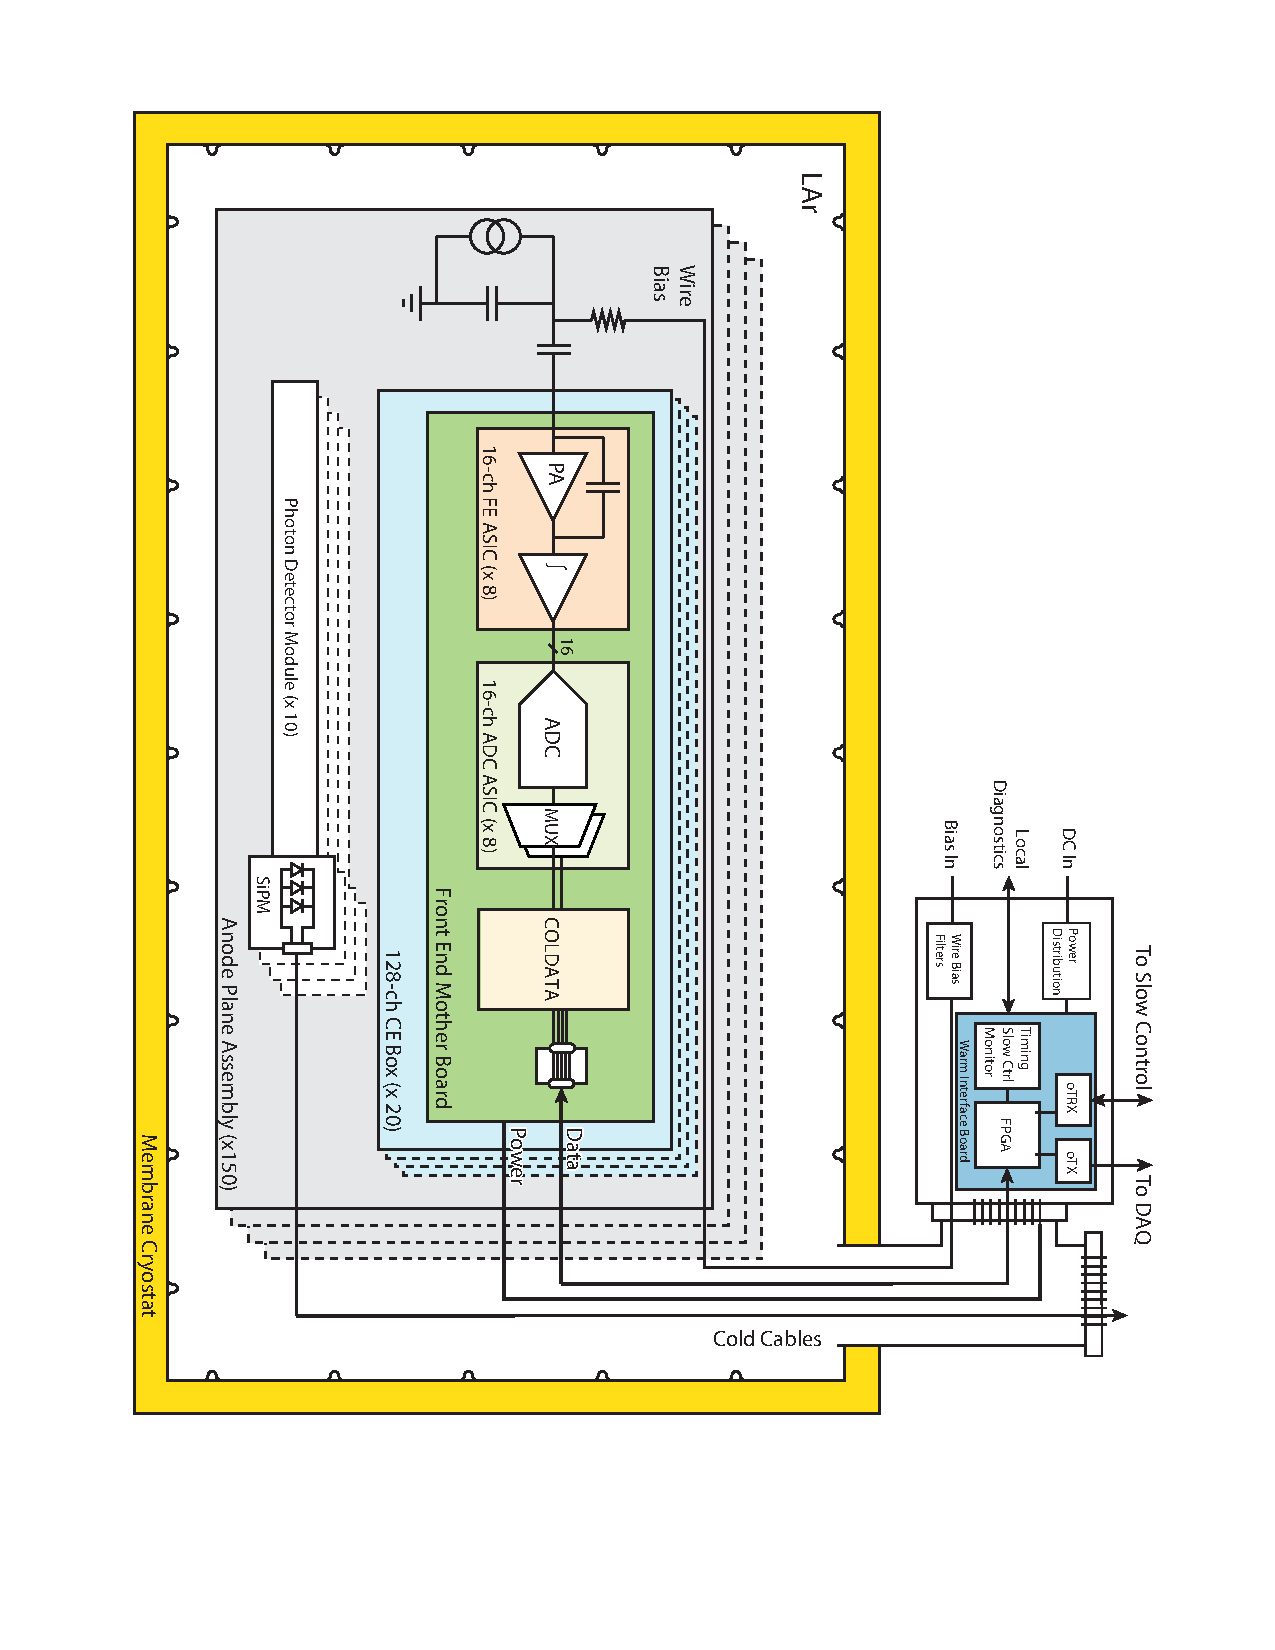
\includegraphics[width=0.9\linewidth,angle=90]{sp-tpcelec-schematic-v3.pdf}
\end{dunefigure}

The \dword{pdsp} version of the \dword{femb} (which uses a single \dword{fpga} on a mezzanine card instead of two \dword{coldata} \dwords{asic}) is shown in Figure~\ref{fig:femb}.

\begin{dunefigure}
[The complete \dword{femb} assembly as used in \dword{pdsp}.]
{fig:femb}
{The complete \dword{femb} assembly as used in the \dword{pdsp} detector. The cable shown is the high-speed data, clock, and control cable.}
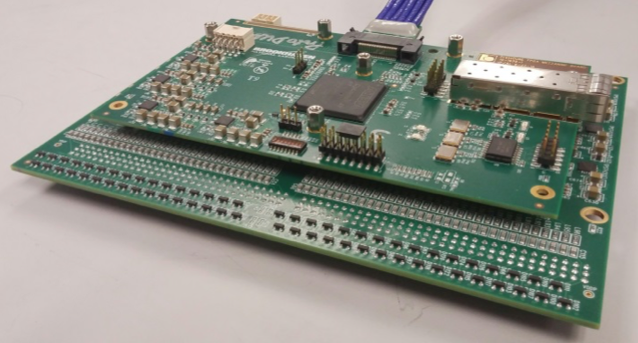
\includegraphics[width=0.6\linewidth]{sp-tpcelec-femb.png}
\end{dunefigure}

%%%%%%%%%%%%%%%%%%
\subsubsection{Front-End ASIC}
\label{sec:fdsp-tpcelec-design-femb-fe}

The analog front-end (FE) ASIC~\cite{DeGeronimo:2011zz} receives current signals from the TPC sense wires and provides a means to amplify and shape the signals for downstream signal digitization.  The FE ASIC has 16 channels, and is implemented using the TSMC 180nm CMOS process. It integrates a band-gap reference (BGR) to generate all the internal bias voltages and currents. This guarantees a high stability of the operating point over a wide range of temperatures, including cryogenic temperatures. The channel schematic of the FE ASIC is shown in Figure~\ref{fig:feasic1}. 

\begin{dunefigure}
[FE ASIC channel schematic]
{fig:feasic1}
{Channel schematic of FE ASIC, which includes a dual-stage charge amplifier and a 5$^{th}$ order semi-Gaussian shaper with complex conjugate poles. Circuits in red circles are programmable to allow different gain and peaking time settings.}
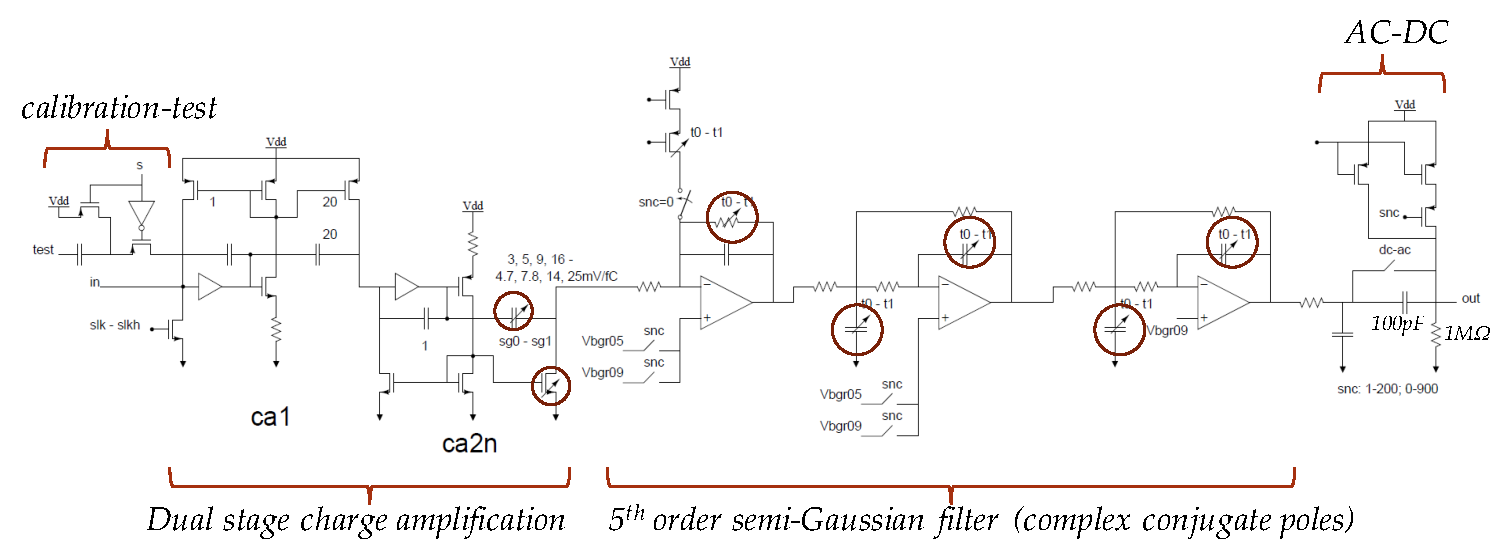
\includegraphics[width=0.99\linewidth]{sp-tpcelec-feasic-channelschematic.pdf}
\end{dunefigure}

Each FE ASIC channel has a dual-stage charge amplifier and a 5$^{th}$ order semi-Gaussian shaper as an anti-aliasing filter for the TPC signals. It has a programmable gain selectable from one of 4.7, 7.8, 14 or 25mV/fC (corresponding to full-scale charge of 300, 180, 100 and 55 fC), a programmable peaking time selectable from one of 0.5, 1, 2, and 3 $\mu$s, and a programmable baseline for operation with either the collection ($\sim$200mV) or the induction ($\sim$900mV) wires. Each channel has an option to enable the output monitor to probe the analog signal, and an option to enable a high-performance output driver that can be used to drive a long cable. 

Each FE ASIC channel has a built-in charge calibration capacitor which can be enabled or disabled through a dedicated register. The injection capacitance has been measured using a calibrated external capacitor. The measurements show that the calibration capacitance is extremely stable, changing from 184 fF at room temperature to 183 fF at 77 K. This result and the measured stability of the peaking time demonstrate the high stability of the passive components as a function of temperature. Channel-to-channel and chip-to-chip variation in the calibration capacitor are typically less than 1\%.

Shared among the 16 channels in the FE ASIC are the digital interface, programming registers, a temperature monitor and a bandgap reference monitor. It also has an option to enable AC coupling as mitigation of microphonics, a programmable bias current selectable from one of 0.1, 0.5, 1 or 5nA, and a programmable pulser generator with 6-bit DAC for calibration. 

The power dissipation of FE ASIC is about 5.5mW per channel at 1.8V supply voltage with output buffer disabled. The ASIC is packaged in a commercial, fully encapsulated plastic QFP 80 package. Figure~\ref{fig:feasic2} shows the response of FE ASIC for all gains and peaking times and both baselines. Note that the gain is independent of the peaking time; the same amount of charge produces the same peak voltage signal regardless of the peaking time.

\begin{dunefigure}
[FE ASIC response and layout]
{fig:feasic2}
{Response of FE ASIC for four gains, four peaking times, and both baseline values (left); layout of 16-channel FE ASIC version P3, where revisions with reference to version P2 are highlighted in yellow boxes (right).}
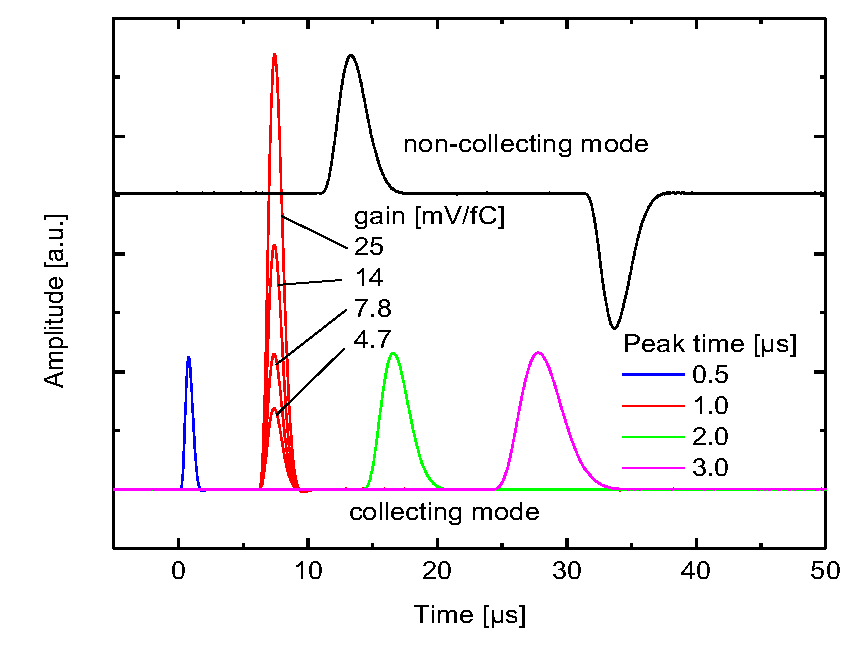
\includegraphics[width=0.48\linewidth]{sp-tpcelec-feasic-response.pdf}
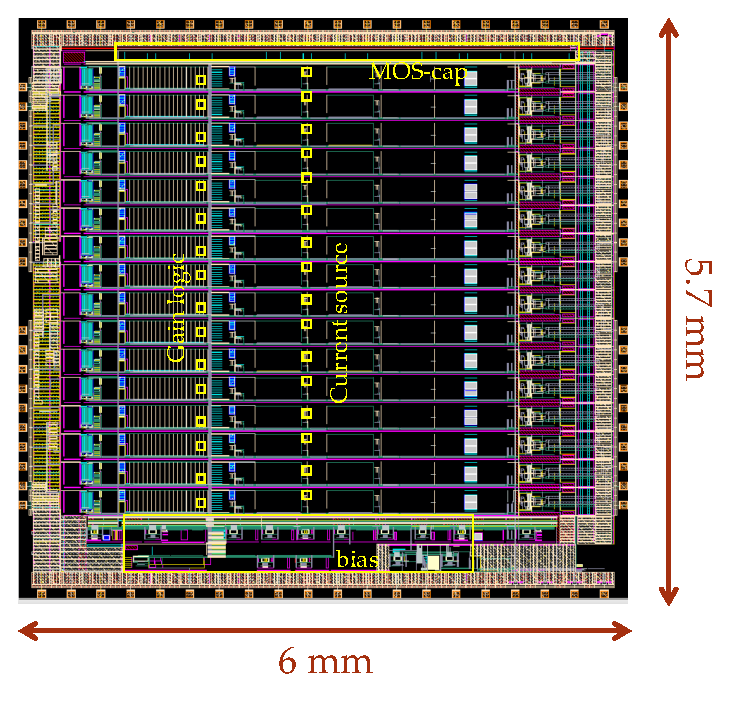
\includegraphics[width=0.48\linewidth]{sp-tpcelec-feasic-layout.pdf}
\end{dunefigure}

Prototype version P2 FE ASICs have been evaluated and characterized at room temperature and LN$_2$ (77 K) temperature. 960 P2 FE ASICs, total 15,360 channels, have been used to instrument six ProtoDUNE-SP APAs successfully. Due to exessive stress of package of FE ASIC in cryogenic temperature, FE channels have non-uniform baseline in collection mode, while the baseline DC voltage in induction mode is uniform. A new prototype version P3 has been fabricated in March 2018 to address this issue by making DC circuits for collection mode similar to the induction mode. At the same time, the default gain setting is changed to 14mV/fC. The layout of P3 FE ASIC is shown in \ref{fig:feasic2}, with modifications highlighted in yellow boxes. The P3 FE ASICs have been received and evaluated in September 2018, which shows both baseline in collection mode and default gain setting are working properly.

P3 FE ASIC will be further evaluated on FEMBs in various integration test stands for performance studies, including 40\% APA at BNL, ICEBERG TPC at Fermilab and APA7 at CERN. Test results of P3 FE ASIC will guide the development of next version P4 FE ASIC, which currently has a plan to implement single ended to differential (SE-DIFF) converter for interface to recently developed ADC ASIC. During the ProtoDUNE-SP operation, it was observed that the FE ASICs may enter into a saturation mode when large amount of charge ($>$ 50fC) is collected in the period of 10-50$\mu$s. This is being studied in the lab test stand, with the plan to address it in the P4 FE ASIC revision as well.

%%%%%%%%%%%%%%%%%%
\subsubsection{ADC ASIC}
\label{sec:fdsp-tpcelec-design-femb-adc}

%%%%%%%%%%%%%%%%%%
\subsubsection{COLDATA ASIC}
\label{sec:fdsp-tpcelec-design-femb-coldata}

%%%%%%%%%%%%%%%%%%
\subsubsection{Alternative Designs}
\label{sec:fdsp-tpcelec-design-femb-alt}

%%%%%%%%%
\subsubsubsection{CRYO Option}
\label{sec:fdsp-tpcelec-design-femb-alt-cryo}

The SLAC CRYO \dword{asic} differs from the baseline three-chip design in that it combines the functions of an analog preamplifier, \dword{adc}, and data serialization and transmission for \num{64}~wire channels, into a single chip.
It is based on a design developed for the nEXO experiment\footnote{Enriched Xenon Observatory, \url{https://www-project.slac.stanford.edu/exo/about.html}.} and differs from it only in the design of the preamplifier, which is modified to account for the higher capacitance of the DUNE \dword{spmod} wires compared to the small pads of nEXO.
The \dwords{femb} constructed using this chip would use only two \dwords{asic}, compared to the \num{18} (eight~FE, eight~\dword{adc} and two~COLDATA) needed in the baseline design.
This drastic reduction in part count may significantly improve \dword{femb} reliablity, reduce power, and reduce costs related to production and testing. 

Figure~\ref{fig:cryo-architecture} shows the overall architecture of the CRYO \dword{asic}, which will be implemented in \SI{130}{nm} \dword{cmos}.
It comprises two identical, \num{32}-channel blocks. 
The current signal from each wire is amplified using a preamplifier with pole zero cancellation and an anti-alias fifth-order Bessel filter applied. 
Provisions are also made for injection of test pulses. 
Gain and peaking time are adjustable to values similar to those of the baseline design.

\begin{dunefigure}
[Overall architecture of the CRYO \dword{asic}.]
{fig:cryo-architecture}
{Overall architecture of the CRYO \dword{asic}.}
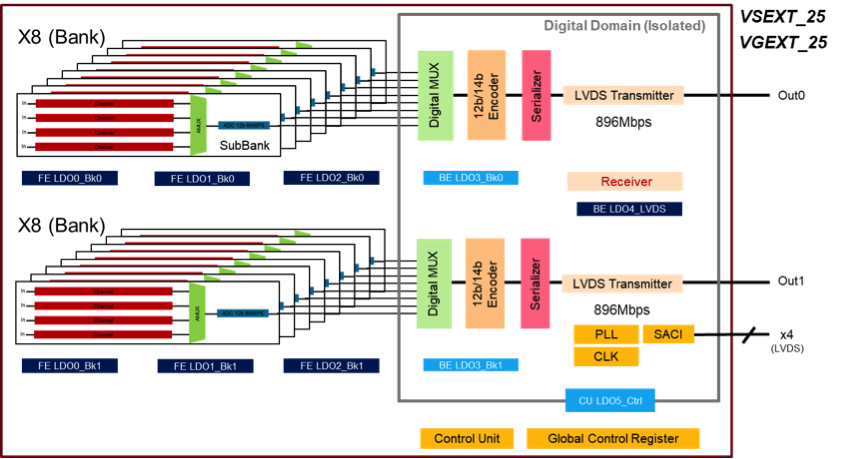
\includegraphics[width=0.8\textwidth]{sp-tpcelec-cryo-schematic.png}
\end{dunefigure}

The \dword{adc} uses \SI{8}{MHz} successive approximation registration (SAR), so that four input channels are multiplexed onto a single \dword{adc}. The data serialization and transmission block employs a custom 12b/14b encoder, so that \num{32} channels of \num{12}-bit, \SI{2}{MHz} data can be transmitted with a digital bandwidth of only \SI{896}{Mbps}, which is significantly less than the required bandwidth of the baseline, which is \SI{1.28}{Gbps}.

One key concern with mixed signal \dwords{asic} is the possibility of interference from the digital side causing noise on the very sensitive preamplifier. 
Fortunately, there are well established techniques for substrate isolation described in the literature~\cite{yeh}, which have been successfully employed in previous \dwords{asic} produced by the SLAC group.% Figure \ref{fig:cryo-substrate} shows how substrate isolation is achieved. 

%\begin{dunefigure}
%[Depiction of the substrate isolation technique that allows combining analog and digital circuitry on the same CRYO \dword{asic}.]
%{fig:cryo-substrate}
%{Depiction of the substrate isolation technique that allows combining analog and digital circuitry on the same CRYO \dword{asic}.}
%\includegraphics[width=0.6\textwidth]{tpcelec-cryo_substrate.png}
%\end{dunefigure}

The infrastructure requirements for a CYRO \dword{asic}-based system are similar to those of the baseline option. However, in most cases, somewhat fewer resources are needed:
\begin{itemize}
\item{A single voltage is needed for the power supply. This is used to generate two supply voltages using internal voltage regulators.}
\item{The output digital bandwidth on each of the four lines in an \dword{femb} is \SI{896}{Mbps}. This is lower than the baseline option due to the custom 12b/14b encoder of the CRYO chip. }
\item{The warm interface is different. Only a single clock is needed (\SI{56}{MHz}) and the configuration protocol is the SLAC \dword{asic} Control Interface (SACI)~\cite{SACI} rather than I2C.}
\end{itemize}

The first iteration of the CRYO \dword{asic} design was submitted for fabrication to MOSIS in November 2018.  The first protoypes are expected to be received in January, 2019. Simulation-based studies have already been performed; at \SI{0.8}{\micro\second} peaking time and an input capacitance of \SI{200}{pF} (similar to that expected in the DUNE \dword{spmod}), the \dword{enc} is approximately \num{500}\,e$^-$.  This noise level is similar to that expected with the baseline \dword{fe} and \dword{adc} \dword{asic} design in \lar with the same input capacitance.  Submission to the \dword{asic} foundry is imminent and the first prototypes should be received by summer 2018. They will first be tested in an existing test stand at SLAC. Subsequent tests are planned for a small test TPC at \fnal and on an \dword{apa} in the \dword{pdsp} cold box; these test facilities are described in Section~\ref{sec:fdsp-tpcelec-qa-facilities}.

In January 2019, stand-alone tests of the CRYO \dword{asic} will begin. In addition to standard ``bringing-up'' tests, measurements of noise (Equivalent Noise Charge), linearity (Equivalent Number of Bits) and bit-error rate will be performed. Figure~\ref{fig:cryo-results} shows ``place-holder'' plots of the type that will be produced in the initial stand-alone tests.

\begin{dunefigure}
[Results of stand-alone tests of the CRYO \dword{asic}.]
{fig:cryo-results}
{Results of stand-alone tests of the CRYO \dword{asic}. Top row shows Equivalent Noise Charge measured in each channel at room temperature (left) and Liquid Nitrogen Temperature (right). Bottom row shows the Equivalent Number of Bits (ENOB). }
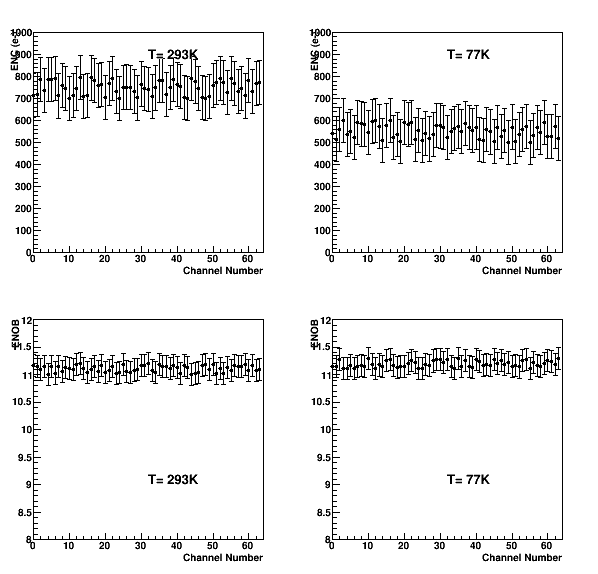
\includegraphics[width=0.8\textwidth]{sp-tpcelec-cryo-results.png}
\end{dunefigure}

%%%%%%%%%
\subsubsubsection{COTS ADC Option}
\label{sec:fdsp-tpcelec-design-femb-alt-cots}

The SBND collaboration has been exploring the COTS (``Commercial Off The Shelf'') ADC option for the TPC readout electronics development since Spring 2017~\cite{Chen:2018zic}. Market survey was carried out, few candidate ADCs in SAR architecture were identified with 100\% cold yield. Since July 2017, a lifetime study plan was developed to evaluate COTS ADC in two different phases, exploratory phase and validation phase. The lifetime study was focused on the ADI AD7274 implemented in TSMC 350nm CMOS technology given the optimum performance in cryogenic operation compared to other candidates.

During the exploratory phase, fresh samples of COTS ADC AD7274 were stressed with higher than nominal operation voltage, such as 5 V, while power consumption (current drawn) was monitored continuously. Periodically the sample would be operated at nominal voltage (V$_{DD}$ = 2.5V and V$_{REF}$ = 1.8V) for performance characterization test, where both DNL (Differential Non-Linearity) and INL (Integral Non-Linearity) were monitored and analyzed in addition to the current monitoring. Stress test results were used to extrapolate the lifetime of the COTS ADC. It was determined that the current drop of 1\% on the V$_{DD}$ is used as degradation criteria for lifetime study. In the validation phase, more devices have been tested following the criteria developed, to collect more data to validate what was learned in the exploratory phase.

The lifetime projection of COTS ADC AD7274 from the stress test with V$_{DD} >$ 5V is shown in Figure~\ref{fig:cotsadc-lifetime}. With ADC7274 operated at 2.5V which is less than the nominal 3.6V for 350nm CMOS technology, the projected lifetime is more than than 10$^6$ years.

\begin{dunefigure}
[Lifetime projection of COTS ADC]
{fig:cotsadc-lifetime}
{Lifetime projection of COTS ADC AD7274 from the stress test with V$_{DD} >$ 5V. The current drop of 1\% on the V$_{DD}$ is used as degradation criteria. With nominal operation voltage of 3.6V for 350nm CMOS technology, the lifetime is projected more than 100 years. For SBND and DUNE far detector, the AD7274 will be operated at 2.5V to gain further margin, the expected lifetime is more than 10$^6$ years.}
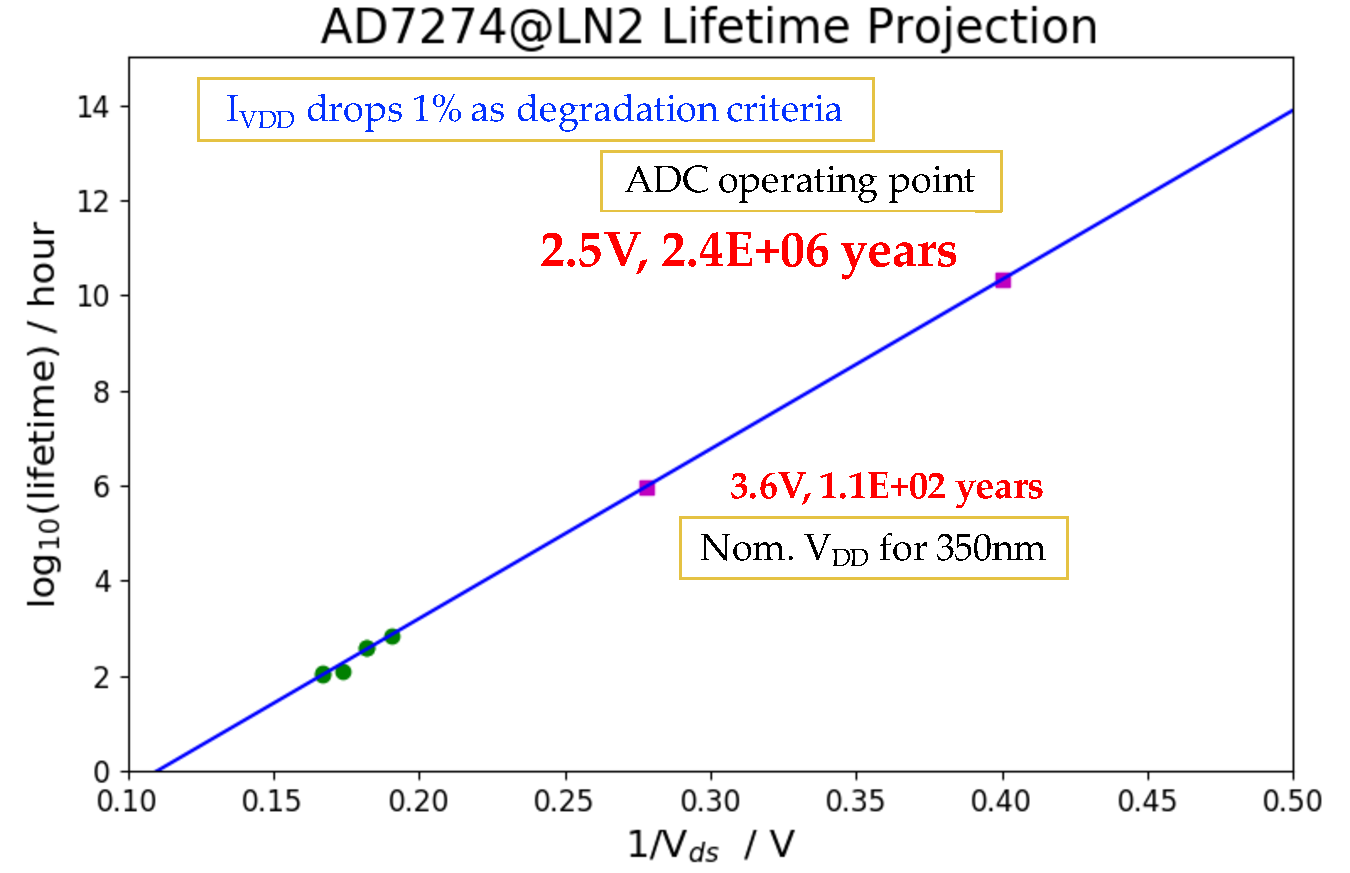
\includegraphics[width=0.8\linewidth]{sp-tpcelec-cotsadc-lifetime.pdf}
\end{dunefigure}

Based on the lifetime study of AD7274, an FEMB with COTS ADC has been developed and characterized for SBND experiment. The integration test was carried out with 40\% APA at BNL and showed satisfactory noise performance in Figure~\ref{fig:cotsadc-fembenc}. The COTS ADC AD7274 serves as a backup solution for DUNE far detector TPC readout electronics system. The current plan is to evaluate it in the small TPC ICEBERG at Fermilab. Ten FEMBs with COTS ADC are being produced and will be used to instrument ICEBERG TPC for system integration test in early 2019. 

\begin{dunefigure}
[ENC measurement of FEMB with COTS ADC]
{fig:cotsadc-fembenc}
{The ENC measurement of FEMB with COTS ADC mounted on 40\% APA at BNL. The picture of FEMB is shown in the top left corner. The induction plane (4 m wire) has ENC $\sim$ 400$e^-$ with 1$\mu$s peaking time, and the collection plane (2.8 m wire) has ENC $\sim$ 330$e^-$ with 1$\mu$s peaking time.}
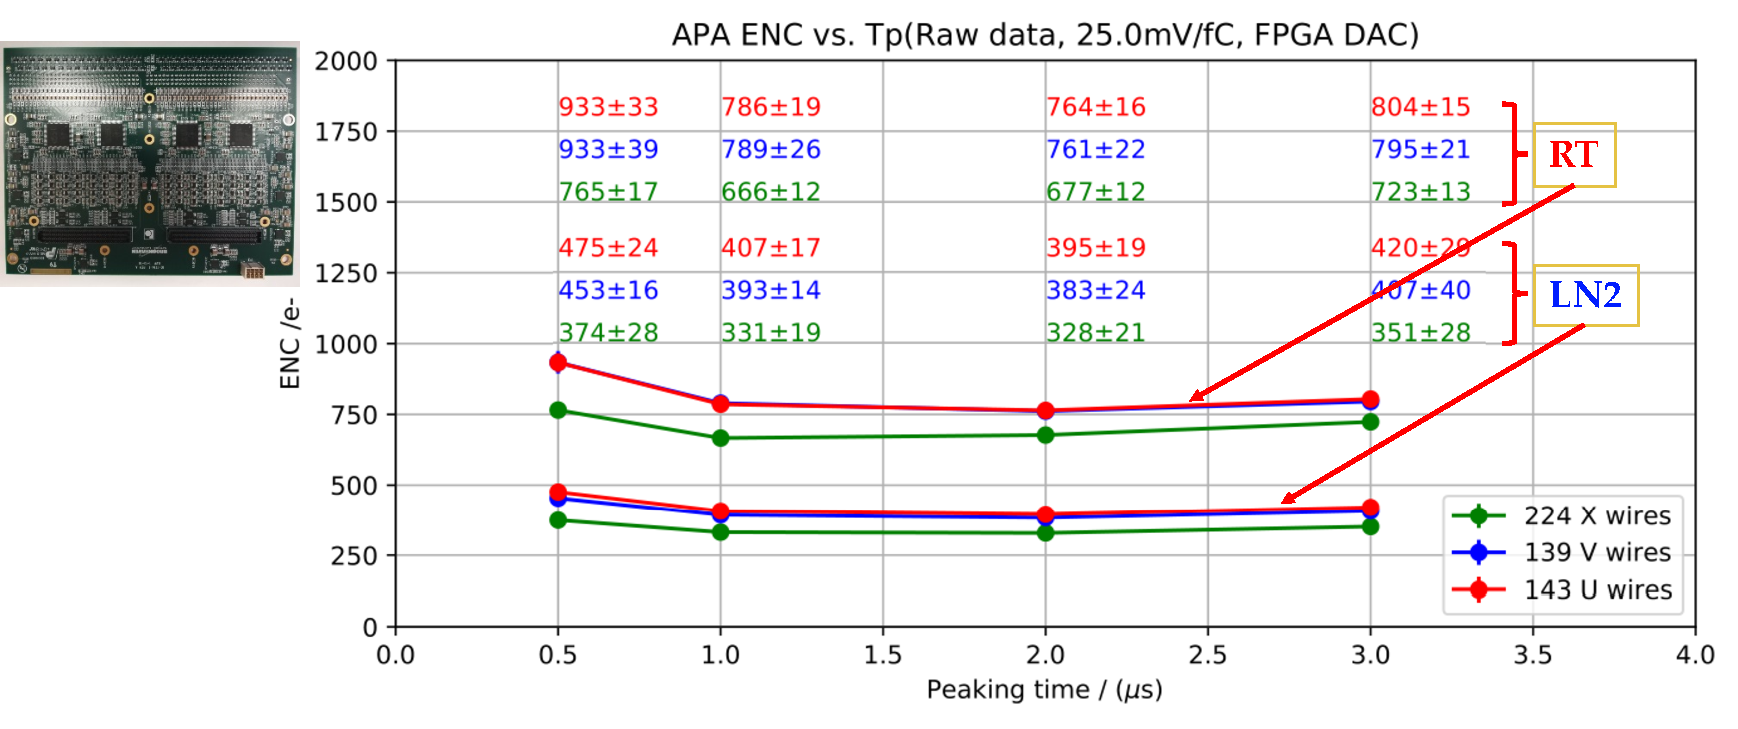
\includegraphics[width=0.99\linewidth]{sp-tpcelec-cotsadc-fembenc.pdf}
\end{dunefigure}

%%%%%%%%%%%%%%%%%%
\subsubsection{Procedure and Timeline for ASIC Selection}
\label{sec:fdsp-tpcelec-design-femb-selection}

%%%%%%%%%%%%%%%%%%%%%%%%%%%%%%%%%%%
\subsection{Infrastructure Inside the Cryostat}
\label{sec:fdsp-tpcelec-design-infrastructure}

%%%%%%%%%%%%%%%%%%%%%%%%%%%%%%%%%%%
\subsection{Cold Electronics Feedthroughs}
\label{sec:fdsp-tpcelec-design-ft}

%%%%%%%%%%%%%%%%%%%%%%%%%%%%%%%%%%%
\subsection{Warm Interface Electronics}
\label{sec:fdsp-tpcelec-design-warm}

%%%%%%%%%%%%%%%%%%%%%%%%%%%%%%%%%%%
\subsection{Services on Top of the Cryostat}
\label{sec:fdsp-tpcelec-design-services}
